\documentclass[12pt,a4paper]{article} 

\usepackage{amsmath,amsfonts,amssymb,latexsym,graphicx,array}
\usepackage[french]{babel}
\usepackage[T1]{fontenc} 
\usepackage[utf8]{inputenc}
\usepackage{color}
\usepackage[a4paper, margin={3cm, 3cm}]{geometry}
\usepackage{subfigure}
\usepackage{epstopdf}
\usepackage{ragged2e}


\begin{document}
%%%%%%%%%%%%%%%%%%%%%%%%%%%%%%%%%%%%%%%%%%%%%%%%%%%%%%%%%%%%%%%%%%%%%%%%%%%%%%%%%%%%%%%%%%%%%
% page titre
%%%%%%%%%%%%%%%%%%%%%%%%%%%%%%%%%%%%%%%%%%%%%%%%%%%%%%%%%%%%%%%%%%%%%%%%%%%%%%%%%%%%%%%%%%%%%
\setcounter{page}{0}


\begin{center}

% logo
\begin{minipage}[l]{.2\linewidth}
	\flushleft
\includegraphics[width=4cm]{img/logo_ENSTA.jpg}
\end{minipage}
\begin{minipage}[r]{.35\linewidth}
	\flushright
\includegraphics[width=4cm]{img/logo_CNAM.png}
\end{minipage}
\begin{minipage}[r]{.3\linewidth}
	\flushright
\includegraphics[width=4cm]{img/logo_X.jpg}
\end{minipage}
\vspace{1.5cm}

% titre
\hrule \vspace{0.5cm}
\begin{LARGE}
	\textbf{RODD-Lot sizing}\\
\end{LARGE}
\vspace{0.5cm} \hrule
\vspace{3cm}

% noms
\definecolor{carmine}{rgb}{0.59, 0.0, 0.09}
\begin{Large}\color{carmine}
	Changmin WU\\
	Ling MA\\
\end{Large}
\vspace{5cm}

% Nom écoles
\begin{large}
	\textit{Conservatoire National des Arts et Métiers\\
	--\\
	\'Ecole Polytechnique\\
	--\\
	\'Ecole Nationale Supérieure de Techniques Avancées\\}
\end{large}
\vfill

% date
\today
\end{center}

\thispagestyle{empty}
\newpage

%%%%%%%%%%%%%%%%%%%%%%%%%%%%%%%%%%%%%%%%%%%%%%%%%%%%%%%%%%%%%%%%%%%%%%%%%%%%%%%%%%%%%%%%%%%%%
%%%%%%%%%%%%%%%%%%%%%%%%%%%%%%%%%%%%%%%%%%%%%%%%%%%%%%%%%%%%%%%%%%%%%%%%%%%%%%%%%%%%%%%%%%%%%

\section{Définition du modèle}
\[
	min\qquad \sum_{m=1}^M \sum_{t=1}^T (p_t^mx_t^m + f_t^my_t^m)+ \sum_{t=1}^T h_t(s_t)
\]

\[
	s.c.\qquad \sum_{m=1}^M x_t^m - s_t+s_{t-1}=d_t\qquad \forall i \in [\![1,n]\!]
\]
\[
	\qquad \qquad \qquad \qquad x_t^m<=(\sum_{t'=t}^T d_{t'})y_t^m\qquad \forall t \in [\![1,T]\!],\forall m \in [\![1,M]\!]
\]
\[
	\qquad \sum_{t'=t}^{t+R-1}\sum_{m=1}^M(e_{t'}^m-E_{t'}^{max})x_{t'}^m<=0\qquad \forall t \in [\![1,T-R+1]\!],\forall m \in [\![1,M]\!]
\]

\begin{flushright}
Cas particuliers:\newline
[R=1]: Contrainte périod;\newline
[R=T]:Contrainte global;\newline
\end{flushright}


Pour le contrainte glissant,  par example: si R=8, on a
\[
	\qquad \sum_{t'=1}^{8}\sum_{m=1}^M(e_{t'}^m-E^{max}_{t'})x_{t'}^m<=0\qquad \forall m \in [\![1,M]\!]
\]

\[
	\qquad \sum_{t'=2}^{9}\sum_{m=1}^M(e_{t'}^m-E^{max}_{t'})x_{t'}^m<=0\qquad \forall m \in [\![1,M]\!]
\]

\[
	\qquad \sum_{t'=3}^{10}\sum_{m=1}^M(e_{t'}^m-E^{max}_{t'})x_{t'}^m<=0\qquad \forall m \in [\![1,M]\!]
\]
\newpage
\section{Analyser le coût total et la valeur de l'émissoin carbone moyenne}

 \begin{minipage}[r]{.99\linewidth}
	\center\includegraphics[width=12cm]{img/10-4-3/10-4-3.png}
\begin{center}
Cette solution est donné par une dt avec une distribution uniform :
[20,25,30,35,40,45,50,55,60,65]
\end{center}

\end{minipage}
\begin{minipage}[b]{.48\linewidth}
	\center\includegraphics[width=7cm]{img/10-4-3/10-4-3-1.png}
	\begin{center}
	[40,30,20,50,34,53,66,80,23,31]
	\end{center}
\end{minipage}
\begin{minipage}[b]{.48\linewidth}
	\center\includegraphics[width=7cm]{img/10-4-3/10-4-3-2.png}
	\begin{center}
	[45,38,23,56,22,56,43,56,65,66]
\end{center}
\end{minipage}
\section{Analyser les résultats}
\begin{justify}
D'abord, On sait que $f_m=[10,30,60,90],e_m=[8,6,4,2]$, c'est à dire, le mode qui émit plus de carbone cout mois chèr. L'objective contient un coût fixé de production et un coût de stockage. Car $h_t=1$, le coût fixé influence plus le l'objective.
\end{justify}
\begin{justify}
Le change de distribution uniform ne change pas la tendance. Pour réspecter le contrainte carbone, il faut choisir plein de fois le mode 4 avec $f_4$=90,$e_4$=2 qui a le plus petit émission mais cout le plus chèr. Si on peut choisir d'autre modes qui sont moins chèrs, cela améliorera nos objective. Pour R=1, il faut choisir 10(T=10) fois de mode 4. Alors R=1 toujours a le coût total le plus haut.
\end{justify}
\begin{justify}
1) En général, le coût total a une tendance d'abord diminuer et ensuit augement quand R augement. Le coût le plus haut est quand le longeur d'intervalle est fixé à 1. Car il faut vérifier le contrainte d'émission carbone par chaque pas de temps et il existe pas de compensation entre les périods.Quand le horizon glissant de longeur fixé devient plus grand, on peut compenser l'émission entre une plus grande intervalle, le bound pour un pas de temps  est relâché, on peut lancer les modes qui émittent plus de carbone qui coute moins chèrs dans une période, si l'émission de quelques périods dépassent le limit d'émission, on peut quand même vérifer la contrainte par diminuer ceux des autres périods pour obtenir une solution optimal.
\end{justify}
\begin{justify}
2) En général, l'émission carbone moyenne a une tendance d'abord augumenter et ensuit diminuer un peu quand R augement. L'émisson le plus bas est quand le longeur d'intervalle est fixé à 1. Car il n'y a pas de compensation entre les périods, chaque pas de temps, on ne peut pas émitter plus de carbone que le limit. Mais quand R augement, le bound pour un pas de temps est relâché grâce à la compensation , pour obtenir un coût minimum, one peut  on peut lancer les modes qui émittent plus de carbone qui coute moins chèrs dans un pas de temps, si l'émission de quelques périods dépassent le limit d'émission, on peut quand même vérifer la contrainte par diminuer ceux des autres périods. 
\end{justify}
\begin{justify}
3) En général, le coût total a une tendance qui inverse la tendance de l'émission carbone moyenne. C'est à dire que on peut éconimiser plus par choisir les modes qui émittent plus de carbone.
\end{justify}
\begin{justify}
4) Le coût total le plus bas l'émission le plus haut sont à R=8.
\end{justify}
\newpage
\section{Analyser l'impact}
\begin{justify}
1) La tendance de coût total ne change pas avec le changement d' Emax,T,M. Le coût total va d'abord diminuer et ensuit augementer.  Et solutionde R du coût total le plus petit devient plus petit.Et solution de R du coût total le plus grand est toujour R=1.
Plus généralement, quand le R augement,  le coût total devient plus petit.
\end{justify}
\begin{justify}
2)
La tendance de l'émission moyenne ne change pas avec le changement d' Emax . L'émission moyenne va d'abord augementer ensuit diminuer.  Et la solutionde R de l'émission  moyenne le plus grand devient plus petit. Et la solution de R de l'émission moyenne le plus petit est toujour R=1.
Plus généralement, quand le R augement, l'émission moyenne plus grand. 
\end{justify}
\begin{justify}
3) La relation entre le coût et l'émission: En général, le coût total a une tendance qui inverse la tendance de l'émission carbone moyenne.
\end{justify}
\subsection{La limit de émission carbone moyenne}
 \begin{minipage}[r]{.99\linewidth}
	\center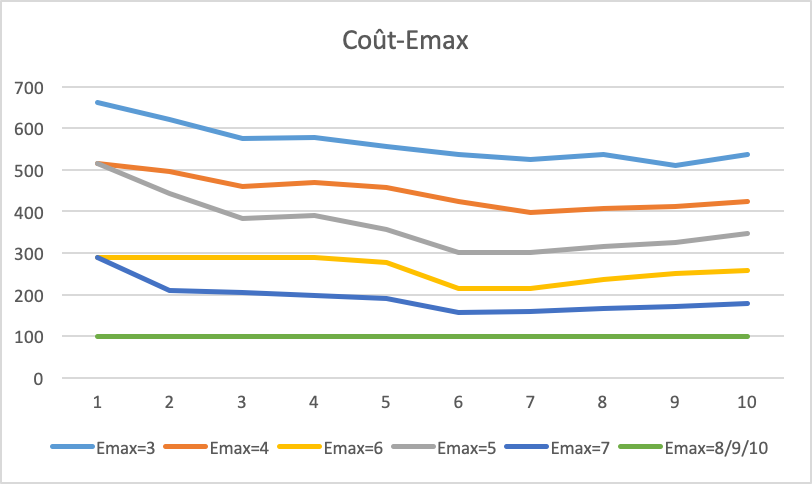
\includegraphics[width=12cm]{img/change/cout-emax.png}
\begin{center}
	\end{center}
\end{minipage}

\begin{minipage}[r]{.99\linewidth}
	\center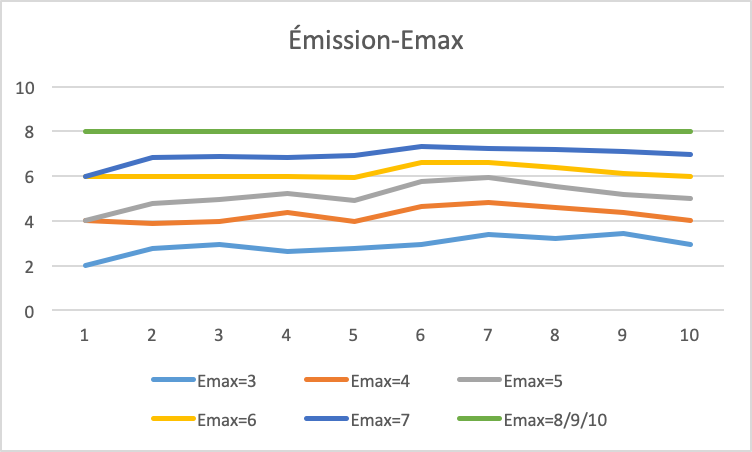
\includegraphics[width=12cm]{img/change/emission-emax.png}
	\begin{center}
	\end{center}
\end{minipage}

\begin{justify}
On suppose T=10, M=4, dt=[40,55,46,35,44,65,20,29,60,47] fixé, on change seulement Emax de 3 ç à 10. Le x-axis est longeur fixé d'intervalle R. Le y-axis de graphe de Coût-Eax est l'objective de modèle, le y-axis de graphe d'Émission-Emax est la limit de l'émission carbone moyenne .
\end{justify}
\begin{justify}
1) Coût : 
 Quand le Emax augement, en général, le coût total pour chaque R diminue. Et quand Emax>=8, le coût ne change plus et est toujours équal à 100. 100 est une borne inférieur du coût total.
\end{justify}
\begin{justify}
2) Émission: Quand le Emax augement, en général, l'émission moyenne augement pour chaque R . Et quand Emax>=8, le coût ne change plus et est toujours équal à 8. 8 est une borne supérieur de la limit d'émission carbon.
\end{justify}

\begin{justify}
3) Raison: Quand Emax=max($e_m$),la bonne supérieur la limit d'émission carbon est le max($e_m$), la borne inférieur du coût total est le T*min($f_m$), car le R=1, il peut vérifer le contrainte d'émission carbone, si le R=1 peut vérifier ce contrainte, les autres longeur qui a une compensation peuvent tous vérifier le contrainte d'émission carbon. On peut choisir le mode qui a min($f_m$) pour tous les $t \subset T$. Alors on peut toujours vérifer le contrainte $\sum_{t'=2}^{9}\sum_{m=1}^M(e_{t'}^m-E^{max}_{t'})x_{t'}^m<=0$ et mettre $s_t$=0. Alors, on peut obtenir la borne inférieur.
\end{justify}
\newpage
\subsection{nombre de mode}
\begin{minipage}[r]{.99\linewidth}
	\center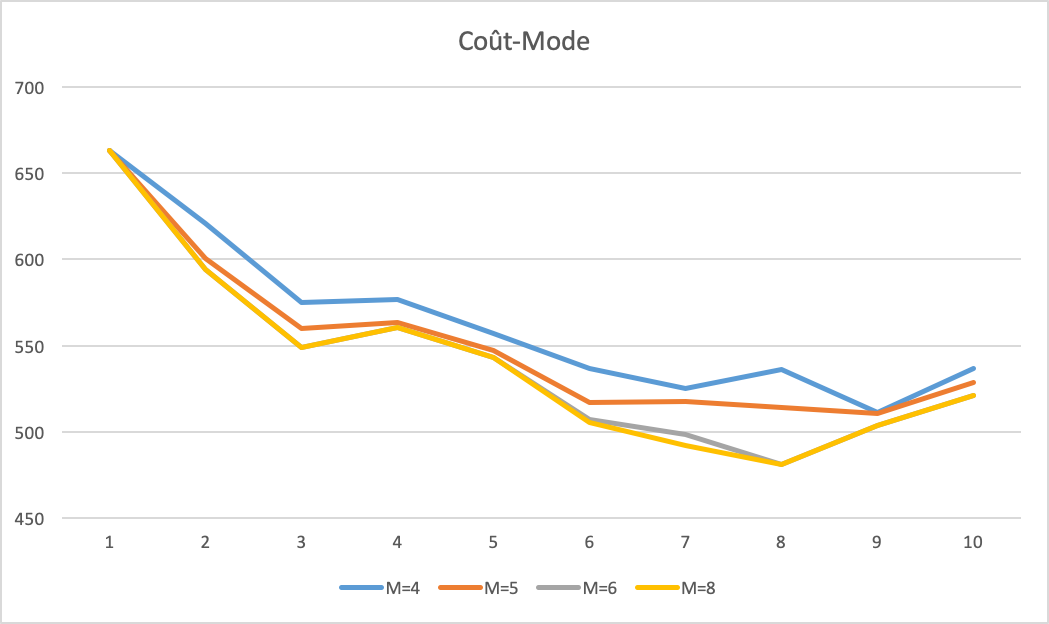
\includegraphics[width=12cm]{img/change/mode-cout.png}
	\begin{center}
	\end{center}
\end{minipage}

\begin{minipage}[r]{.99\linewidth}
	\center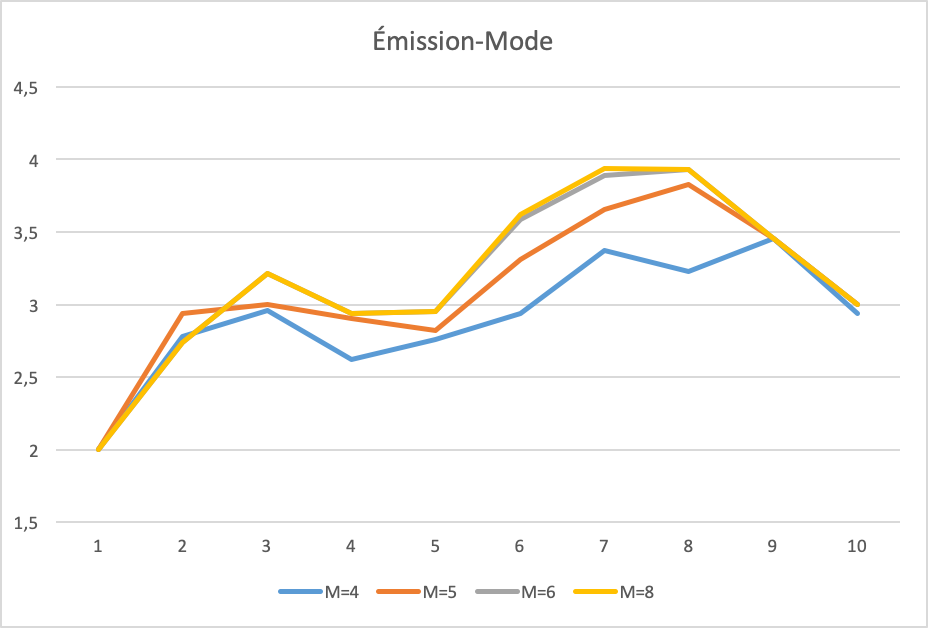
\includegraphics[width=12cm]{img/change/mode-emission.png}
	\begin{center}
	\end{center}
\end{minipage}
\begin{justify}
On suppose T=10, Emax=3, dt=[40,55,46,35,44,65,20,29,60,47] fixé, on change seulement M de 4 à 10. On ajoute $f_m$ et $e_m$ pour le nouveau mode par la relation: si $e_m$ est grand, $f_m$ est petit. 
\end{justify}
\begin{justify}
Quand M=9 ou 10, le coût total et l'émission moyenne variant sur R sont les mêmes quand M=8. Le x-axis est longeur fixé d'intervalle R. Le y-axis de graphe de Coût-Mode est l'objective de modèle, le y-axis de graphe d'Émission-Mode est la limit de l'émission carbone moyenne .
\end{justify}
\begin{justify}

1) Coût : Quand le M augement, en général, le coût total pour chaque R diminue un peu mais pas beaucoup. Et quand M>=8, le coût total de chaque R ne diminue plus avec M croissant. 
\end{justify}
\begin{justify}
2) Émission: Quand le M augement, en général, l'émission moyenne augement un peu pour chaque R . Et quand M>=8, l'émission moyenne  de chaque R ne croisse plus avec le M croissant. Et pour le R=T,  l'émission moyenne pour chaque T est Emax. Et pour le R=1,  l'émission moyenne pour chaque T est la même.
\end{justify}
\begin{justify}
3) Raison: Quand M devient plus grand, c'est à dire que on a plus de modes à choisir. On doit toujours réspecter le contraine et choisir le mode qui a plus d'émission mais cout mois chère pour obtenir une meillure solution, plus de modes nous fournissent plus de meillure choix. Mais si les meuillures mode sont déjà dans le M qui vérifient d'autres containtes aussi, ça va pas changer grand chose car on peut seulement faire T choix maximum.
\end{justify}
\newpage
\subsection{longeur de l'horizon}
\begin{minipage}[r]{.99\linewidth}
	\center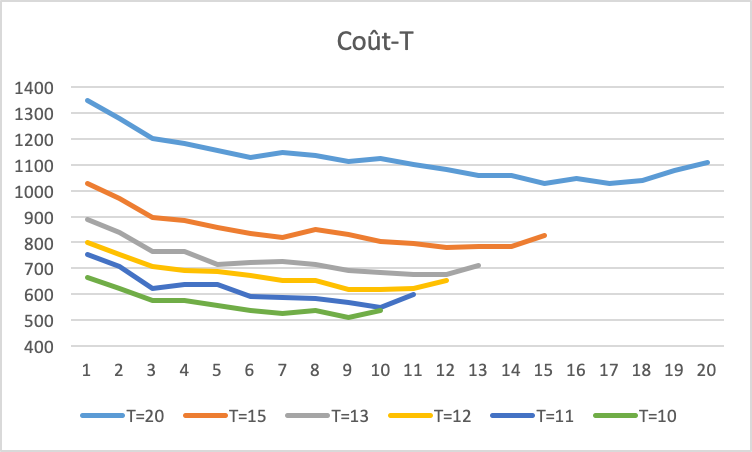
\includegraphics[width=12cm]{img/change/t-cout.png}
	\begin{center}
	\end{center}
\end{minipage}

\begin{minipage}[r]{.99\linewidth}
	\center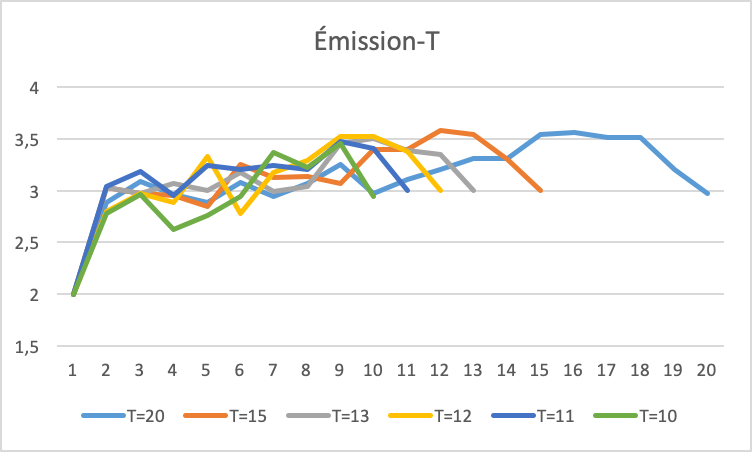
\includegraphics[width=12cm]{img/change/t-emission.png}
	\begin{center}
	\end{center}
\end{minipage}
\begin{justify}
On suppose M=4, Emax=3, dt=[40,55,46,35,44,65,20,29,60,47] fixé, on change seulement T. T=[10,11,12,13,15,20]. Le x-axis est longeur fixé d'intervalle R. Le y-axis de graphe de Coût-T est l'objective de modèle, le y-axis de graphe d'Émission-T est la limit de l'émission carbone moyenne .
\end{justify}
\begin{justify}

1) Coût : Quand le T augement, en général, le coût total pour chaque R augement. 
\end{justify}
\begin{justify}
2) Émission: Quand le T augement, en général, l'émission moyenne devient stable entre [3,3.5]. Et pour le R=T,  l'émission moyenne pour chaque T est Emax. Et pour le R=1,  l'émission moyenne pour chaque T est la même.
\end{justify}
\begin{justify}
3) Raison: Si T devient plus grand, on a plus de demand en total à satisfier, alors le coût total pour chaque R devient plus grand. 
\end{justify}

\section{Conclusion}

Pour conclure, La tendance de coût total ne change pas par R avec le changement d' Emax,T, M. Le coût total va d'abord diminuer et ensuit augementer. Et solution de R du coût total le plus grand est toujour R=1.En général, le coût total a une tendance qui inverse la tendance de l'émission carbone moyenne par chaque R. 

Si Emax croissant, le coût total décroissant, l'émission moyenne croissant. Si T croissant, le coût total croissant, l'émission moyenne devient stable. Si on M croissant, le coût total décroissant et ensuit stable, l'émission moyenne croissant et ensuit stable.

L'objective est déterminé par le coût fixé et le coût de stockage.Car le $h_s$ est 1, l'objective est plutôt déterminé par le coût fixé de mode. Quand le R de a une intervalle plus grand, on a une périod plus longue pour compensation, on peut alors choisir les modes qui ont coût fixé moin chèr mais émittent plus de carbone pour obtenir une solution moin chèr et émit plus de carbone. 

Si on peut avoir un mode qui émit moins de carbone et  cout moin chèr, on peut optimiser notre l'objective.

\end{document}